\documentclass[10pt]{fphw}

% Template-specific packages
\usepackage[utf8]{inputenc} % Required for inputting international characters
\usepackage[T1]{fontenc} % Output font encoding for international characters
%\usepackage{mathpazo} % Use the Palatino font
\usepackage{amsmath}
\usepackage{mathtools}
\usepackage{graphicx} % Required for including images
\usepackage{subcaption}
\usepackage{booktabs} % Required for better horizontal rules in tables
\usepackage{amsthm}
\usepackage{minted}
%\usemintedstyle[R]{friendly}

\usepackage{listings} % Required for insertion of code
\usepackage{hyperref}
\hypersetup{
	colorlinks=true,
	linkcolor=blue!50!red,
}
\usepackage{enumerate} % To modify the enumerate environment

\theoremstyle{definition}
\newtheorem{definition}{Definition}

\newtheorem{theorem}{Theorem}
\newtheorem{corollary}{Corollary}

\title{Homework \#2} % Assignment title
\author{Alex Towell (\href{mailto:atowell@siue.edu}{\bfseries{atowell@siue.edu}})}

\date{02/12/2021} % Due date
\institute{Southern Illinois University-Edwardsville}
\class{STAT 478 - Time Series Analysis}
\professor{Dr. Beidi Qiang}

\newcommand{\var}{\operatorname{Var}}
\newcommand{\expect}{\operatorname{E}}
\newcommand{\corr}{\operatorname{Corr}}
\newcommand{\cov}{\operatorname{Cov}}

\newcommand{\is}[1]{\mathcal{I}_{#1}}
\newcommand{\Is}[1]{\mathcal{I}(#1)}

\newcommand{\eval}[3]{\left. #1 \right\vert_{#2}^{#3}}

\newcommand{\comment}[1]{}

\begin{document}
\maketitle % Output the assignment title, created automatically using the information in the custom commands above
\section*{Question 1}
\begin{problem}
Consider the $N$-span moving average applied to data that is uncorrelated with mean $\mu$ and
variance $\sigma^2$.
\begin{enumerate}
\item[(a)] Show that the variance of the moving average is $\var(M_t) = \sigma^2 /N$.
\item[(b)] Show that $\cov(M_t , M_{t+k}) = \sigma^2
\sum_{j=1}^{N-k}(1/N)^2$.
\item[(c)] Show the ACF is
\begin{equation*}
\rho_k = 1 - \frac{|k|}{N}, \text{for $k < N$.}
\end{equation*}
\end{enumerate}
\end{problem}

\subsection*{Answer}

\begin{enumerate}
\item[(a)] To simplify the presentation of the subsequent material, we define the following parameterized index set.

\begin{definition}
We define $I_t$ to be the index set (of size $N$) given by
\begin{equation}
    \mathcal{I}_t \coloneqq \{ t-N+1,t-N,\ldots,t-1,t \}\,.
\end{equation}
\end{definition}

$M_t$ is defined as
\begin{equation}
    M_t \coloneqq \frac{1}{N} \!\!\sum_{i=t-N+1}^{t}\!\!\!\! Y_i = \frac{1}{N}\sum_{i \in \is{t}} Y_i\,.
\end{equation}

The variance of $M_t$ is given by
\begin{equation}
    \var(M_t) = \var\!\left(\frac{1}{N} \sum_{i \in \is{t}} Y_i\right) = \frac{1}{N^2} \sum_{i \in \is{t}} \var(Y_i)\,.
\end{equation}
It is given that the variance for the time series $\{Y_t\}$ is a constant denoted by $\sigma^2$, therefore
\begin{equation}
    \var(M_t) = \frac{1}{N^2} \sum_{i \in \is{t}} \sigma^2 = \frac{1}{N^2} N \sigma^2 = \frac{\sigma^2}{N}\,.
\end{equation}

\item[(b)] The covariance of $M_t$ and $M_{t+k}$ is given by
\begin{align}
    \cov(M_t,M_{t_k}) &= \expect(M_t M_{t+k}) - \expect(M_t)\expect(M_{t+k})\\
                      &= \expect\left[\left(\frac{1}{N} \sum_{i\in\is{t}} Y_i\right) \left(\frac{1}{N} \sum_{j\in\is{t+k}} Y_j\right)\right] - \mu^2\\
                      &= \frac{1}{N^2}\expect\left[\left(\sum_{i \in \is{t}} Y_i\right) \left(\sum_{j\in\is{t+k}} Y_j\right)\right] - \mu^2\,.
\end{align}

We focus our attention on the following definition.

\begin{definition}
$W$ is expected value given by the sum of products
\begin{align}
    W &\coloneqq \expect\left[\left(\sum_{i\in\is{t}} Y_i\right) \left(\sum_{j\in\is{t+k}} Y_j\right)\right]\\
%      &= \expect\left[Y_{t-N+1} Y_{t+k-N+1} + \cdots + \cdots + Y_t Y_{t+k} \right]\\
      &= \sum_{(i,j) \in S} \expect(Y_i Y_j)\,,
\end{align}
where $S \coloneqq \is{t} \times \is{t+k}$, which is a Cartesian product of cardinality $|S| = N^2$.
\end{definition}

With this definition of $W$, the covariance of $M_t$ and $M_{t+k}$ may be rewritten as
\begin{equation}
    \cov(M_t,M_{t_k}) = \frac{1}{N^2} W - \mu^2\,.
\end{equation}

By the assumption of independence, if $l \neq m$, then
\begin{equation}
\label{eq:indep}
    \expect(Y_l Y_m) = \expect(Y_l) \expect(Y_m) = \mu^2
\end{equation}
and since $\var(Y_l) = \expect(Y_l^2) - \expect^2(Y_l)$,
\begin{equation}
\label{eq:dep}
    \expect(Y_l Y_l) = \expect^2(Y_l) + \var(Y_l) = \mu^2+\sigma^2\,.
\end{equation}

If $k \geq N$, then $M_t$ and $M_{t+k}$ have no components of $\{Y_t\}$ in
common. By eq~\ref{eq:indep}, this means that
\begin{equation}
    W = N^2 \mu^2
\end{equation}
and therefore
\begin{equation}
    \cov(M_t,M_{t+k}) = \frac{1}{N^2} W - \mu^2 = \mu^2 - \mu^2 = 0\,.
\end{equation}

If $k < N$, then $M_t$ and $M_{t+k}$ have some components of $\{Y_t\}$ in
common.
Therefore, $W$ consists of $N-k$ expectations of the form $\expect(Y_l Y_l)$
with the expected value $\mu^2 + \sigma^2$
and $N^2 - (N-k) = N^2 - N + k$ expectations of the form $\expect(Y_l Y_m)$,
$l \neq m$, with the expected value $\mu^2$.
Therefore, $W = (N-k)(\mu^2 + \sigma^2) + (N^2-N+k) \mu^2 = (N-k)\sigma^2 + N^2 \mu^2$.
When we plug this $W$ into the covariance equation, we get the result
\begin{equation}
    \cov(M_t,M_{t_k}) = \frac{1}{N^2}\left((N-k)\sigma^2 + N^2 \mu^2\right) - \mu^2 = \frac{N-k}{N^2}\sigma^2 + \mu^2 - \mu^2 = \frac{N-k}{N^2}\sigma^2
\end{equation}
which may be rewritten as
\begin{equation}
    \cov(M_t,M_{t_k}) = \sigma^2 \sum_{j=1}^{N-k} (1/N)^2\,.
\end{equation}
Observe that if $N-k < 1$, then $\sum_{j=1}^{N-k} (1/N)^2 = 0$, and thus this also covers the case when $k \geq N$ where we earlier proved the covariance is zero.

\item[(c)] In the last problem, we show that the autocovariance is strictly a function of lag $k$ (with $N$ constant). Thus,
$r_k = \frac{N-k}{N^2}\sigma^2$.

The autocorrelation function is given by
\begin{align}
    \rho_k = \frac{r_k}{\var(M_t)}
        &= \frac{\frac{N-k}{N^2}\sigma^2}{\sigma^2/N}\\
        &= \frac{N-k}{N} = 1 - \frac{k}{N}\,.        
\end{align}
Since the autocorrelation function is symmetric, the result is the same whether $k$ is positive or negative, and thus
\begin{equation}
    \rho_k = 1 - \frac{|k|}{N}\,.
\end{equation}
\end{enumerate}


\section*{Question 2}
\begin{problem}
Suppose that $Z_1$ and $Z_2$ are uncorrelated random variables with $\expect(Z_1) = \expect(Z_2) = 0$ and $\var(Z_1) = \var(Z_2) = 1$.
Consider the process defined by
\begin{equation}
    Y_t \coloneqq Z_1 \cos(\omega t) + Z_2 \sin(\omega t) + e_t\,,
\end{equation}
where $e_t$'s are iid and independent of both $Z_1$ and $Z_2$, $e_t \sim \mathcal{N}(0,\sigma^2)$.
\begin{enumerate}
    \item[(a)] Prove that $\{Y_t\}$ is stationary. (Hint: $\cos(\alpha - \beta) = \cos \alpha \cos \beta + \sin \alpha \sin \beta$.)
    \item[(b)] Let $Z_1$ and $Z_2$ be independent $\mathcal{N}(0, 1)$ random variables, and set $\sigma^2 = 1$ and $\omega = 0.5$.
    Use R to simulate $n = 250$ observations from the $\{Y_t\}$ process.
    Plot $\{Y_t\}$ and describe the appearance of your time series.
    \item[(c)] Now consider the process
    \begin{equation*}
        X_t \coloneqq \beta_0 + \beta_1 t + Z_1 \cos \omega t + Z_2 \sin \omega t + e_t\,.
    \end{equation*}
    Show that the time series $\{X_t\}$ is not stationary. Then use R to simulate a realization of $\{X_t\}$.
    Plot $\{X_t\}$ and describe the appearance of your time series. Does your $\{X_t\}$ process appear to be stationary?
    
    \item[(d)] Consider the differenced time series $\{\Delta X_t\}$, where $\Delta X_t \coloneqq X_t-X_{t-1}$.
    Show that the first difference $\{\Delta X_t\}$ is actually stationary. Plot the first differences $\Delta X_t$,
    you may use $\operatorname{diff}$ in R to get the difference. Describe the appearance of this difference process
    $\{\Delta X_t\}$. Does it appear to be stationary?
\end{enumerate}
\end{problem}

\subsection*{Answer}

\begin{enumerate}
\item[(a)] To prove that $\{Y_t\}$ is weakly stationary, it is sufficient to prove that it has a constant mean, a constant variance, and its ACF is strictly a function of lag.
First, observe
\begin{align}
\expect(Y_t) &= \expect(Z_1 \cos(\omega t) + Z_2 \sin(\omega t) + e_t)\\
&= \cos(\omega t) \expect(Z_1) + \sin(\omega t) \expect(Z_2)  + \expect(e_t) = 0
\end{align}
and
\begin{align}
\var(Y_t) &= \var(Z_1 \cos(\omega t) + Z_2 \sin(\omega t) + e_t)\\
&= \cos^2(\omega t) \var(Z_1) + \sin^2(\omega t) \var(Z_2)  + \var(e_t)\\
&= \cos^2(\omega t) + \sin^2(\omega t) + \sigma^2 = 1+\sigma^2\,,
\end{align}
so we see that the mean and variance are constant.

Next, the ACF is given by $\cov(Y_t,Y_{t+k})$. By the properties of the covariance function,
\begin{equation}
\label{eq:cov_prop}
\begin{split}
\cov(a_1 X_1 + a_2 X_2, a_3 X_3 + a_4 X_4) = a_1 a_3 \cov(X_1,X_3) + a_1 a_4 \cov(X_1,X_4) + \\
\qquad a_2 a_3 \cov(X_2,X_3) + a_2 a_4 \cov(X_2, X_4)\,.
\end{split}
\end{equation}

We let $Y_t = a Z_1 + b Z_2 + e_t$ and $Y_{t+k} = c Z_1 + d Z_2 + e_{t+k}$
where $a = \cos(\omega t)$, $b = \sin(\omega t)$, $c = \cos(\omega(t+k))$, and $d = \sin(\omega(t+k))$,
and thus we are interested in
\begin{equation}
    \cov(a Z_1 + b Z_2 + e_t, c Z_1 + d Z_2 + e_{t+k})\,.
\end{equation}
We apply pattern matching to make the above equation match eq~\ref{eq:cov_prop}.
We $X_2 = b Z_2 + e_t$ and $X_4 = d Z_2 + e_{t+k}$, and thus we wish to find
\begin{equation}
    \cov(a Z_1 + X_2, c Z_1 + X_4) = a c \cov(Z_1,Z_1) + a \cov(Z_1,X_4) + c \cov(X_2,Z_1) + \cov(X_2,X_4)\,.
\end{equation}
Observe that $\cov(Z_1,Z_1) = \var(Z_1) = 1$ and $Z_1$ is independent of both $X_4$ and $X_2$, thus we may rewrite
the above as
\begin{equation}
\label{eq:part1}
    \cov(a Z_1 + X_2, c Z_1 + X_4) = a c + \cov(X_2,X_4)\,.
\end{equation}
We now pattern match on $\cov(X_2,X_4)$. Substituting the definitions of $X_2$ and $X_4$,
we see that
\begin{align*}
    \cov(X_2,X_4)
                &= \cov(b Z_2 + e_t, d Z_2 + e_{t+k})\\
                &= b d \cov(Z_2,Z_2) + b \cov(Z_2,e_{t+k}) + d \cov(e_t,Z_2) + \cov(e_t,e_{t+k})\,.
\end{align*}
Observe that $\cov(Z_2,Z_2) = \var(Z_2) = 1$ and $Z_2$ is independent of both $e_t$ and $e_{t+k}$, thus we may rewrite
the above as
\begin{equation}
\label{eq:part2}
    \cov(X_2,X_4) = b d + \cov(e_t,e_{t+k})\,.
\end{equation}
When we combine eq~\ref{eq:part2} with eq~\ref{eq:part1}, we get the result
\begin{equation}
    \cov(a Z_1 + b Z_2 + e_t, c Z_1 + d Z_2 + e_{t+k}) = a c + b d + \cov(e_t,e_{t+k})\,.
\end{equation}
If $k = 0$, then $\cov(e_t,e_t) = \var(e_t) = \sigma^2$ and otherwise if $k\neq 0$ then $\cov(e_t,e_{t+k}) = 0$ by independence.

%Since $a = \cos(\omega t)$, $b = \sin(\omega t)$, $c = \cos(\omega(t+k))$, and $d = \sin(\omega(t+k))$,
%$a c + b d = \cos(\omega t) \cos(\omega(t+k)) + \sin(\omega t)\sin(\omega(t+k))$.

By the trigometric idenity $\cos (\alpha - \beta) = \cos \alpha \cos \beta + \sin \alpha \sin \beta$, if we let $\alpha = \omega t$ and $\beta = \omega(t+k)$,
we may rewrite $a c + b d$ as $\cos(-\omega k)$ since $\alpha - \beta = \omega t - \omega(t+k) = \omega(t - (t+k)) = -\omega k$.
By the property that $\cos(-a) = \cos(a)$, we may finally rewrite $a c + b c$ to $\cos(\omega k)$.

Putting all of this together, we arrive at
\begin{equation}
    r_k = \cov(Y_t,Y_{t+k}) = \cos(\omega k)
\end{equation}
if $k \neq 0$ and
\begin{equation}
    r_0 = \var(Y_t) = 1 + \sigma^2\,,
\end{equation}
which is in agreement with our earlier more direct computation of the variance.
By the fact that the mean is a constant $0$, the variance $\var(Y_t) = r_0$ is a constant $1 + \sigma^2$, and the ACF is strictly a function of lag,
we may conclude that $\{Y_t\}$ satisfies the requirements of being weakly stationary.

\fbox{Note to Dr. Q: I have another proof that directly uses $\cov(Y_t,Y_{t+k}) = \expect(Y_t Y_{t+k})$.}

\item[(b)] Figure~\ref{fig:plot2b} is a plot of $\{Y_t\}$ with $n=250$, $\sigma^2 = 1$, and $\omega = 0.5$ using R script in listing~\ref{lst:plot2b}. 
The variance appears constant, but it does exhibit seasonality despite the fact that we proved it has a
constant mean and autocovariance that is strictly a function of lag.

There is a white noise component $e_t$, but there is also a sinusoidal component.
Each realization of a time series is sinusoidal with a random amplitude and random phase.
Suppose $\{Y_t\}^{(i)}$ is defined as
\begin{align}
    Y_t^{(i)} &\coloneqq Z_{i,1} \cos(\omega t) + Z_{i,2} \sin(\omega t) + e_{i,t}\\
              &= \sqrt{Z_{i,1}^2+Z_{i,2}^2} \cos(\omega t - \arctan(Z_{i,2}/Z_{i,1})) + e_{i,t}\,,
\end{align}
where $Z_{i,1},Z_{i,2} \sim \mathcal{N}(0,1)$ for all $i$ and $e_{i,t} \sim \mathcal{N}(0,\sigma^2)$.
Then, $\expect(Y_t^{(i)}) = 0$ for all $i$ but any particular realization of $Z_{i,1}$ and $Z_{i,2}$ will
be non-zero and thus will have a seasonable trend. For instance, given that $Z_{i,1} = a$ and $Z_{i,2} = b$,
$Y_t^{(i)}$ has an expected value $a \cos(\omega t) + b \sin(\omega t)$ which is a function of time $t$.

We compare two different realizations of the time series in fig~\ref{fig:plot2b_cmp}.

It is interesting to note there is zero correlation between independent time series $\{Y_t\}^{(i)}$ and $\{Y_t\}^{(j)}$, $j \neq j$,
since they have random phases.

%\begin{figure}[h]
%    \centering
%    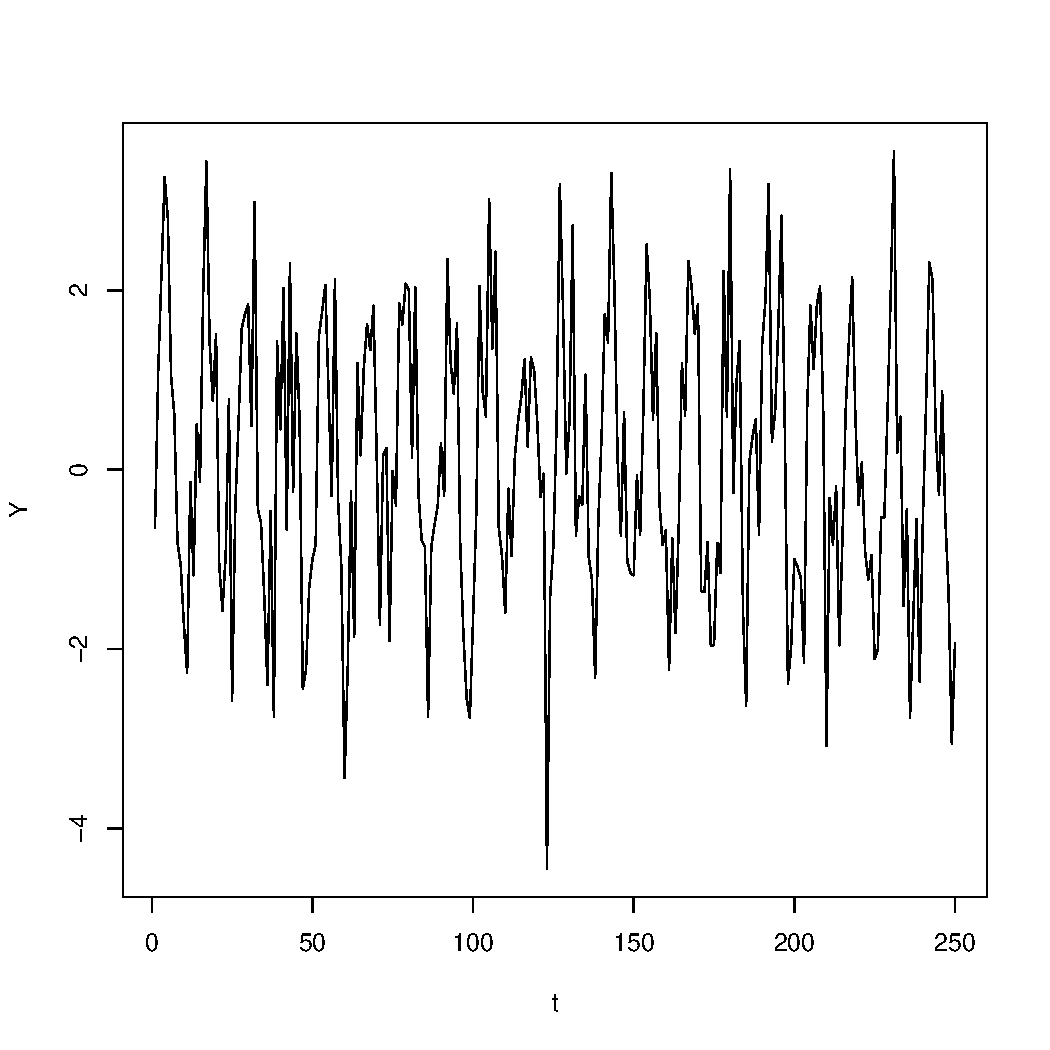
\includegraphics[width=.5\linewidth]{plot2_b_orig}
%    \caption{Time series plot of $\{Y_t\}$.}
%    \label{fig:plot2b}
%\end{figure}
%
%In fig~\ref{fig:plot2b_cmp}, we show two independent
%realizations of the time series, $\{Y_t\}^{(1)}$ and $\{Y_t\}^{(2)}$.
%\begin{figure}[h]
%\centering
%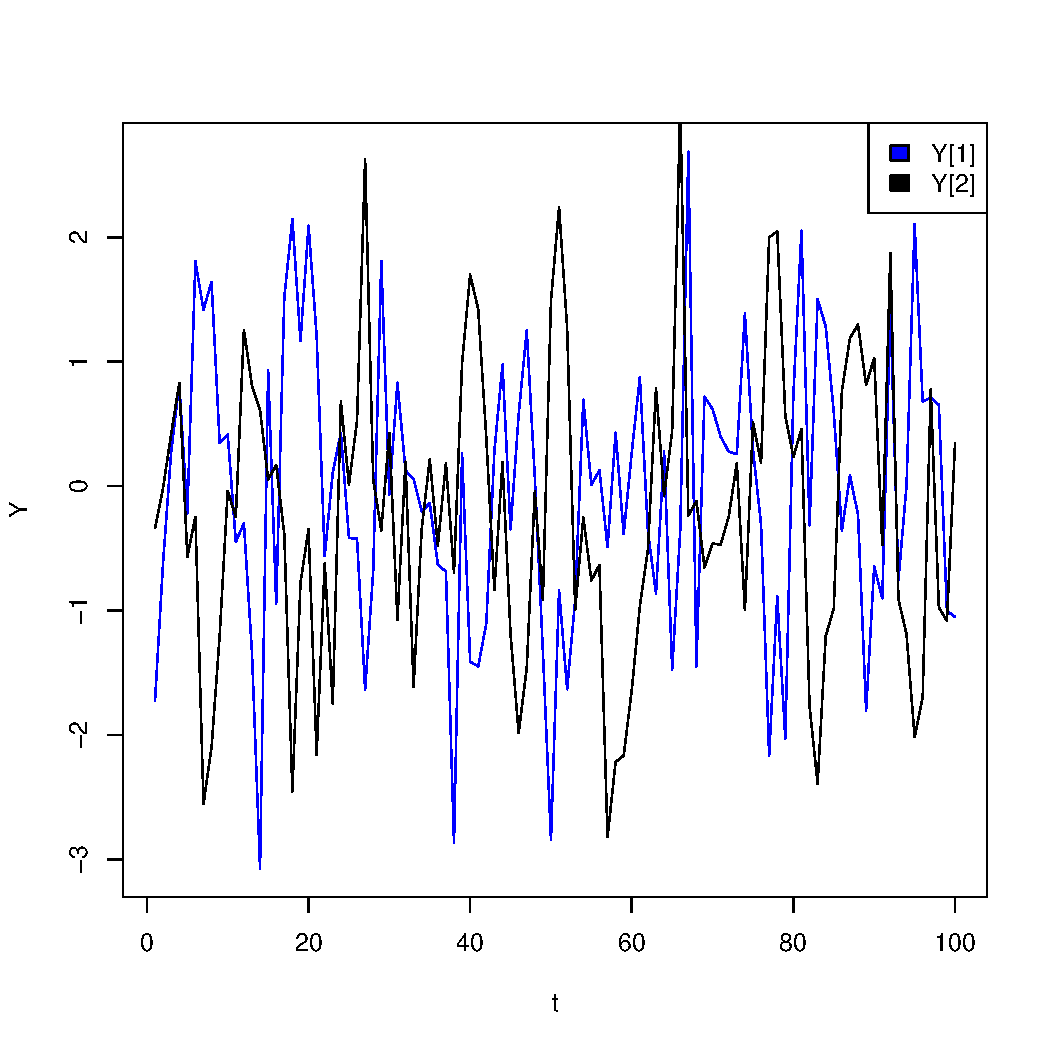
\includegraphics[width=.5\linewidth]{plot2_b}
%\caption{Time series plot of $\{Y_t\}$.}
%\label{fig:plot2b_cmp}
%\end{figure}

\begin{listing}
\caption{R script used to generate time series plots for $Y_t$.}
\label{lst:plot2b}
\begin{minted}
[
fontsize=\footnotesize,
mathescape,
linenos,
breaklines,
frame=lines,
framesep=2mm
]{r}
# homework #2: problem 2.b

# n is size of time series
n <- 250

w <- 0.5

# $Z_1,Z_2 \sim \mathcal{N}(0,1)$
z <- rnorm(2, mean=0,sd=1)

# white noise ${e_t} \sim \mathcal{N}(0,1)$
e <- rnorm(n, mean=0,sd=1)

# ${Y_t}$ is the time series of interest
Y <- vector(length=n)

for (t in 1:n)
{
    Y[t] = z[1]*cos(w*t) + z[2]*sin(w*t) + e[t]
}

pdf(file="plot2_b_orig.pdf")
plot(Y,type="l", xlab="t", ylab="Y")
\end{minted}
\end{listing}

\begin{figure}
    \centering
    \begin{subfigure}{.5\textwidth}
        \centering
        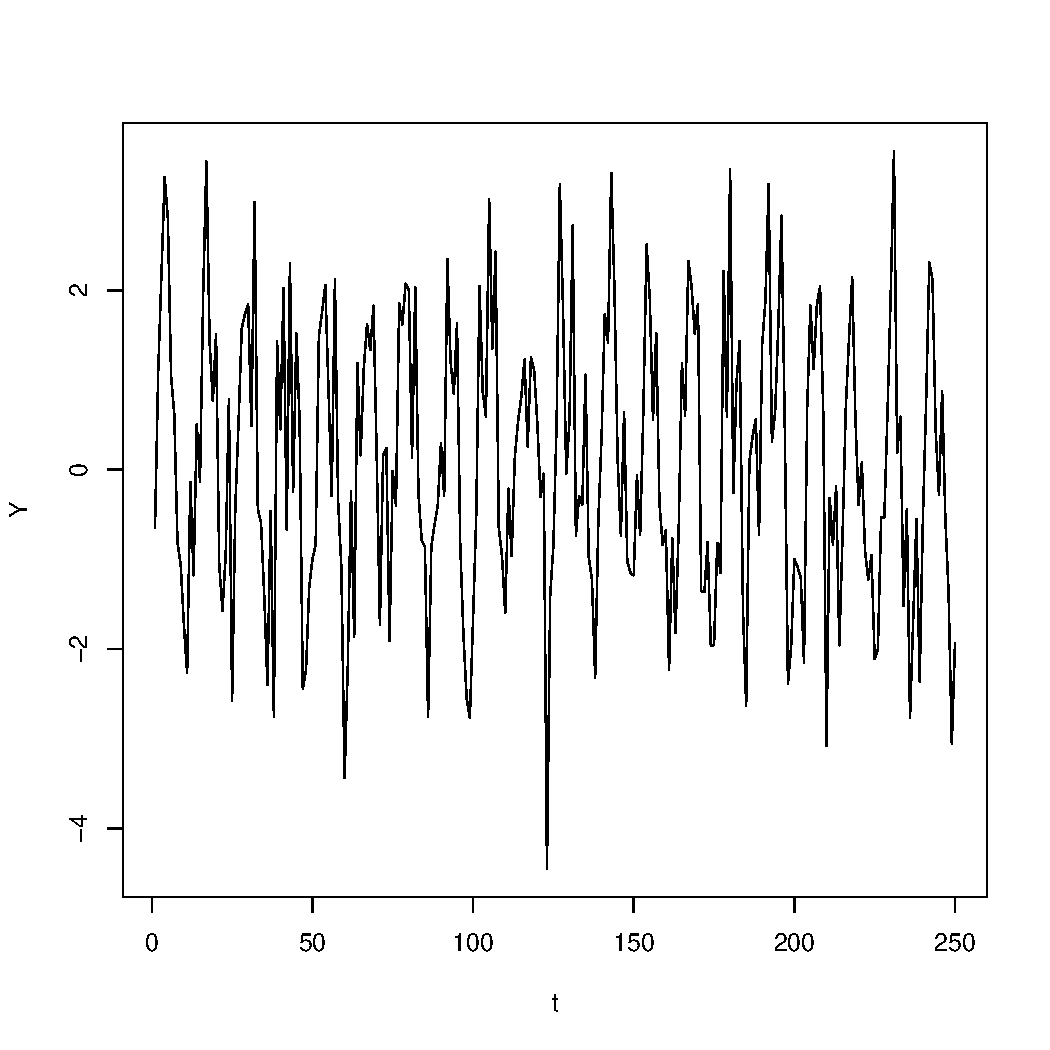
\includegraphics[width=.85\linewidth]{plot2_b_orig}
    \caption{Time series plot of $\{Y_t\}$.}
    \label{fig:plot2b}
    \end{subfigure}%
    \begin{subfigure}{.5\textwidth}
        \centering
        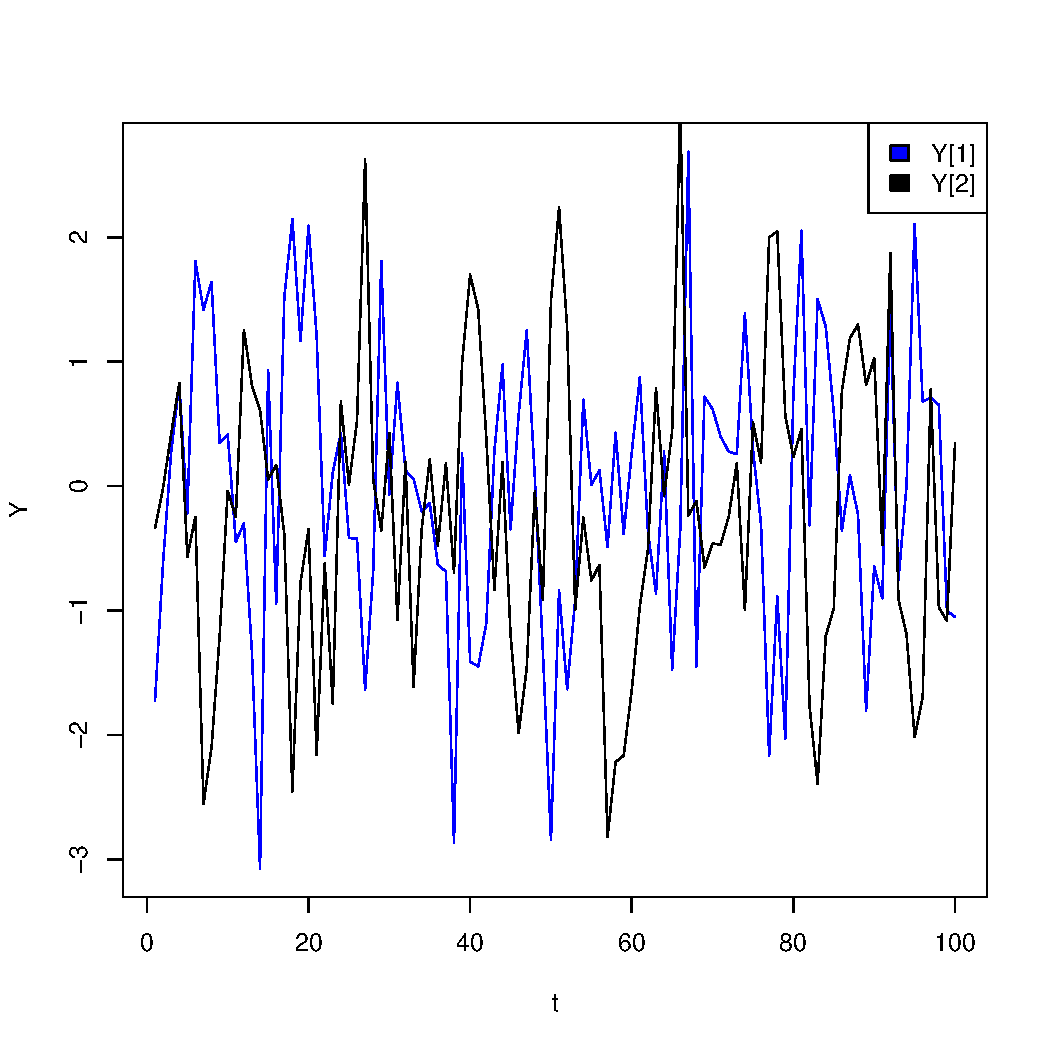
\includegraphics[width=.85\linewidth]{plot2_b}
    \caption{Comparison of time series plot of $\{Y_t\}^{(1)}$ and $\{Y_t\}^{(2)}$.}
    \label{fig:plot2b_cmp}
    \end{subfigure}
\end{figure}



\item[(c)] $X_t$ is defined as
\begin{equation}
    X_t \coloneqq \beta_0 + \beta_1 t + Z_1 \cos \omega t + Z_2 \sin \omega t + e_t\,.
\end{equation}

For $\{X_t\}$ to be stationary, one of the conditions is that it must have a constant mean.
The expectation of $X_t$ is given by
\begin{align}
    \expect(X_t)
        &= \expect(\beta_0 + \beta_1 t + Z_1 \cos \omega t + Z_2 \sin \omega t + e_t)\\
        &= \beta_0 + \beta_1 t + \cos \omega t \expect(Z_1) + \sin \omega t \expect(Z_2) + \expect(e_t)\\
        &= \beta_0 + \beta_1 t\,,
\end{align}
which is a linear function with respect to time.
Therefore, if $\beta_1 \neq 0$, the mean is a function of time and is non-constant, in which case $\{X_t\}$ is not stationary.

To illustrate, we plot $\{X_t\}$ with $\beta_0 = 0$ and $\beta_1 = 0.05$ in fig~\ref{fig:plot2c}.
Clearly, the time series is positively correlated with time $t$ and thus is non-stationary.
Otherwise, the variance seems to be constant.
Moreover, $X_t = \beta_0 + \beta_1 t + Y_t$, and therefore $\{X_t - \beta_0 - \beta_1 t\} = \{Y_t\}$,
so if we subtract the trendline out of the time series we have a stationary time series.

\begin{figure}
    \centering
    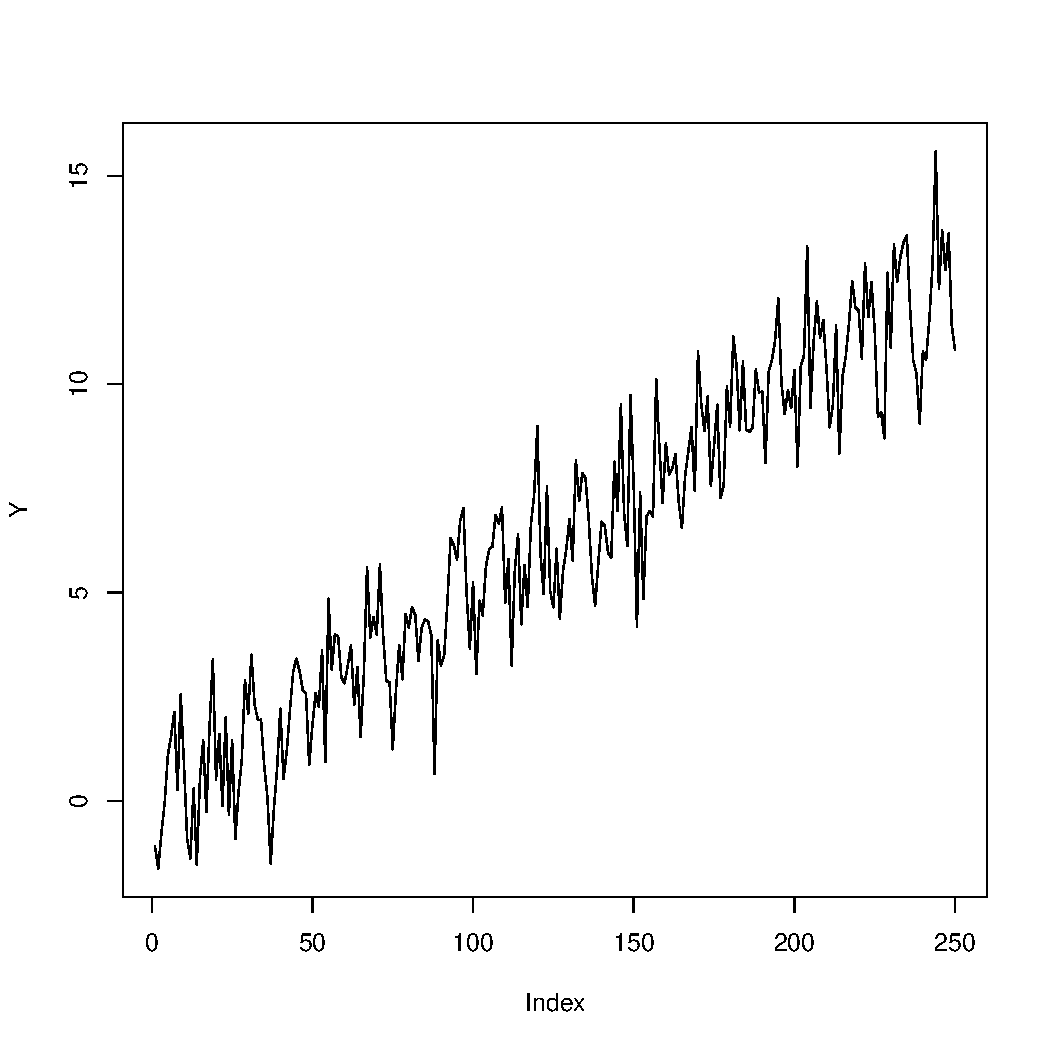
\includegraphics[width=.5\linewidth]{plot2_c}
    \caption{Time series plot of $\{X_t\}$.}
    \label{fig:plot2c}
\end{figure}

\item[(d)] The difference operator $\nabla$ is defined as
\begin{equation}
    \nabla A_t \coloneqq A_t - A_{t-1}\,.
\end{equation}
Therefore, substituting the definition of $X_t$ into the $\nabla$ function results in
\begin{equation*}
\begin{split}
    \nabla X_t
        &\coloneqq X_t - X_{t-1}\\
        &= \left(\beta_0 + \beta_1 t + Z_1 \cos \omega t + Z_2 \sin \omega t + e_t\right) -\\
           &\qquad\left(\beta_0 + \beta_1 (t-1) + Z_1 \cos(\omega (t-1)) + Z_2 \sin(\omega (t-1)) + e_{t-1}\right)\\
%        &= \beta_1 t - \beta_1 (t-1) + Z_1 \cos \omega t - Z_1 \cos(\omega (t-1)) + Z_2 \sin \omega t -\\
%           &\qquad Z_2 \sin(\omega (t-1)) + e_t - e_{t-1}\\
        &= \beta_1 + Z_1 (\cos \omega t - \cos(\omega (t-1))) + Z_2 (\sin \omega t - \sin(\omega (t-1))) + (e_t - e_{t-1})\,.
\end{split}
\end{equation*}
Letting $\operatorname{g}(t) \coloneqq \cos \omega t - \cos(\omega(t-1))$ and $\operatorname{h}(t) \coloneqq \sin \omega t - \sin(\omega(t-1))$,
we rewrite the above as
\begin{equation}
    \nabla X_t = \beta_1 + \operatorname{g}(t) Z_1  + \operatorname{h}(t) Z_2 + (e_t - e_{t-1})\,.
\end{equation}

%Observe that $\nabla e_t = e_t - e_{t-1}$, as the difference of two independent and normally distributed random variables, is normally distributed as
%\begin{equation}
%    \nabla e_t \sim \mathcal{N}(0,2\sigma^2)\,.
%\end{equation}

The expectation and variance of $\nabla X_t$ is given respectively by
\begin{align*}
    \expect(\nabla X_t)
        &= \beta_1 + \operatorname{g}(t) \expect(Z_1) + \operatorname{h}(t) \expect(Z_2) + \expect(e_t) - \expect(e_{t-1})\\
        &= \beta_1 + \operatorname{g}(t) \cdot 0 + \operatorname{h}(t) \cdot 0 + 0 - 0
\end{align*}
and
\begin{align*}
\var(\nabla X_t)
    &= \operatorname{g}^2(t) \var(Z_1) + \operatorname{h^2}(t)\var(Z_2) + \var(e_t) + \var(e_{t-1}))\\
    &= \operatorname{g}^2(t) + \operatorname{h}^2(t) + 2 \sigma^2\\
    &= 2(1+\sigma^2-\cos \omega)\,,
\end{align*}
which are both constants.

The covariance $\cov(\nabla X_t,\nabla X_{t+k})$ is given by
\begin{equation}
\begin{split}
    \cov(\nabla X_t,\nabla X_{t+k}) = \expect
        [
            &(\operatorname{g}(t) Z_1 +
                \operatorname{h}(t) Z_2 + (e_t - e_{t-1}))\\
            &(\operatorname{g}(t+k) Z_1 +
                \operatorname{h}(t+k) Z_2 + (e_{t+k} - e_{t+k-1}))
        ]\,.
\end{split}
\end{equation}

Expanding the inner part of the expectation above results in an expectation of a sum of products.
Taking advantage of the linearity of expectation, we rewrite this as a sum of expectation of products and we
discard those expectations that are unconditionally zero, leaving us with
\begin{equation}
\begin{split}
\cov(\nabla X_t,\nabla X_{t+k}) =
    &\operatorname{g}(t)\operatorname{g}(t+k)\expect(Z^2_1) + \operatorname{h}(t)\operatorname{h}(t+k)\expect(Z^2_2)\\
    &+ \expect(e_t e_{t+k}) - \expect(e_t e_{t+k-1}) - \expect(e_{t-1} e_{t+k}) + \expect(e_{t-1} e_{t+k-1})\,.
\end{split}
\end{equation}
Since $\expect(Z_1^2) = \expect(Z_2^2) = 1$, and assuming $k > 0$, then by the assumption of independence $\expect(e_{t-1} e_{t+k}) = \expect(e_{t-1}) \expect(e_{t+k}) = 0$ and we rewrite the above as
\begin{equation}
\begin{split}
\cov(\nabla X_t,\nabla X_{t+k}) =
    &\operatorname{g}(t)\operatorname{g}(t+k) + \operatorname{h}(t)\operatorname{h}(t+k)\\
    &+ \expect(e_t e_{t+k}) - \expect(e_t e_{t+k-1}) + \expect(e_{t-1} e_{t+k-1})\,,
\end{split}
\end{equation}
which simplies to
\begin{equation}
    \cov(\nabla X_t,\nabla X_{t+k}) = 2(1-\cos\omega) \cos(k \omega) + \expect(e_t e_{t+k}) - \expect(e_t e_{t+k-1}) + \expect(e_{t-1} e_{t+k-1})\,.
\end{equation}

The only point of consideration remaining are the expectations in the above equation.
By independence, $\expect(e_i e_j) = 0$, $i \neq j$, and $\expect(e^2_j) = \sigma^2$.
If $k = 0$, these expectations sum to $2 \sigma^2$.
If $k = 1$, these expectations sum to $\sigma^2$.
Finally, if $k > 1$, these expectations sum to $0$.
Putting it all together, the autocovariance function is given by
\begin{equation}
r_k = -2(\cos\omega-1) \cos(k \omega) + (2-|k|)\sigma^2[|k| < 2]\,,
\end{equation}
where $[p]$ is the Iverson bracket that is $1$ if predicate $p$ is true and otherwise $0$.\footnote{Also, observe that $\cos(-a) = \cos(a)$, so $r_k = r_{-k}$, as expected.}
As expected, $r_0 = \var \Delta X_t$.

We have shown that $\{\Delta X_t\}$ has a constant expectation and variance and the autocovariance $r_k$ is strictly a function of lag $k$.
Thus, $\{\nabla X_t\}$ satisfies the requirements of a weakly stationary time series. In fig~\ref{fig:plot2d}, we show a plot of $\{\Delta X_t\}$,
which seems to be stationary as it jumps around $0$ with a relatively constant variance and no obvious correlations.
\begin{figure}[h]
    \centering
    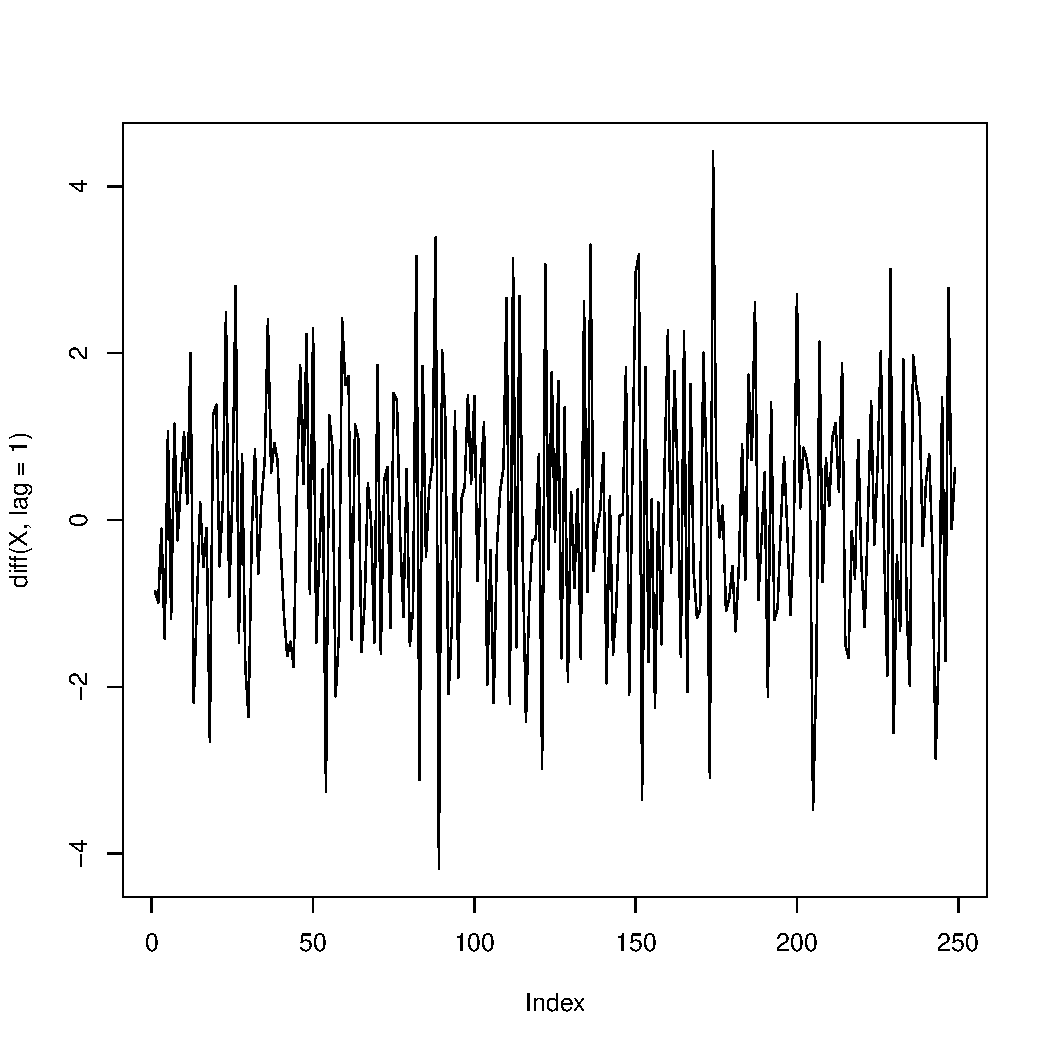
\includegraphics[width=.29\linewidth]{plot2_d}
    \caption{Time series plot of $\{\nabla X_t\}$.}
    \label{fig:plot2d}
\end{figure}
\end{enumerate}


\newpage
\section*{Question 3}
\begin{problem}
The monthly values of the average hourly wages for U.S. apparel and textile workers for July
1981 to June 1987 are in the wages object in the TSA package. Type library(TSA); data(wages);
print(wages) in R to see the data set.
\begin{enumerate}
\item[(a)] Plot the time series. What basic pattern do you see from the plot?
\item[(b)] Fit a linear time trend model using least squares. Give the plot of the linear trend overlain on the
data, and give the estimated regression equation.
\item[(c)] Plot the standardized residuals from the linear regression over time. Comment on any notable
pattern.
\item[(d)] Fit a quadratic time trend model using least squares. Give the plot of the quadratic trend overlain
on the data, and give the estimated regression equation.
\item[(e)] Plot the standardized residuals from the quadratic regression over time. Comment on any notable
pattern.
\end{enumerate}
\end{problem}

\subsection*{Answer}

\begin{enumerate}
    \item[(a)] In fig~\ref{fig:plot3a}, we see a plot of wages with respect to year.
    The dominant feature of this time series is the increasing wages over this time period.
%    The variability in the data seems relatively mild, suggesting a trend of some kind,
%    and what variability is there seems constant.
%   
%    A model that is the best fit \emph{to the data} is probably quadratic, but a line would
%    also be reasonable. Ultimately, if we wish to use the model to make predictions about
%    the future...
    
    \item[(b)] The line of best fit to the \emph{wages} time series dataset is given by
    \begin{equation}
        \hat{\expect}(X_t) \coloneqq 7.93144 + 0.02342 t\,.
    \end{equation}    
    We plot the wages time seres with this line of best fit in fig~\ref{fig:plot3b}.
    
    \begin{figure}
    \begin{subfigure}{.5\textwidth}
    \centering
    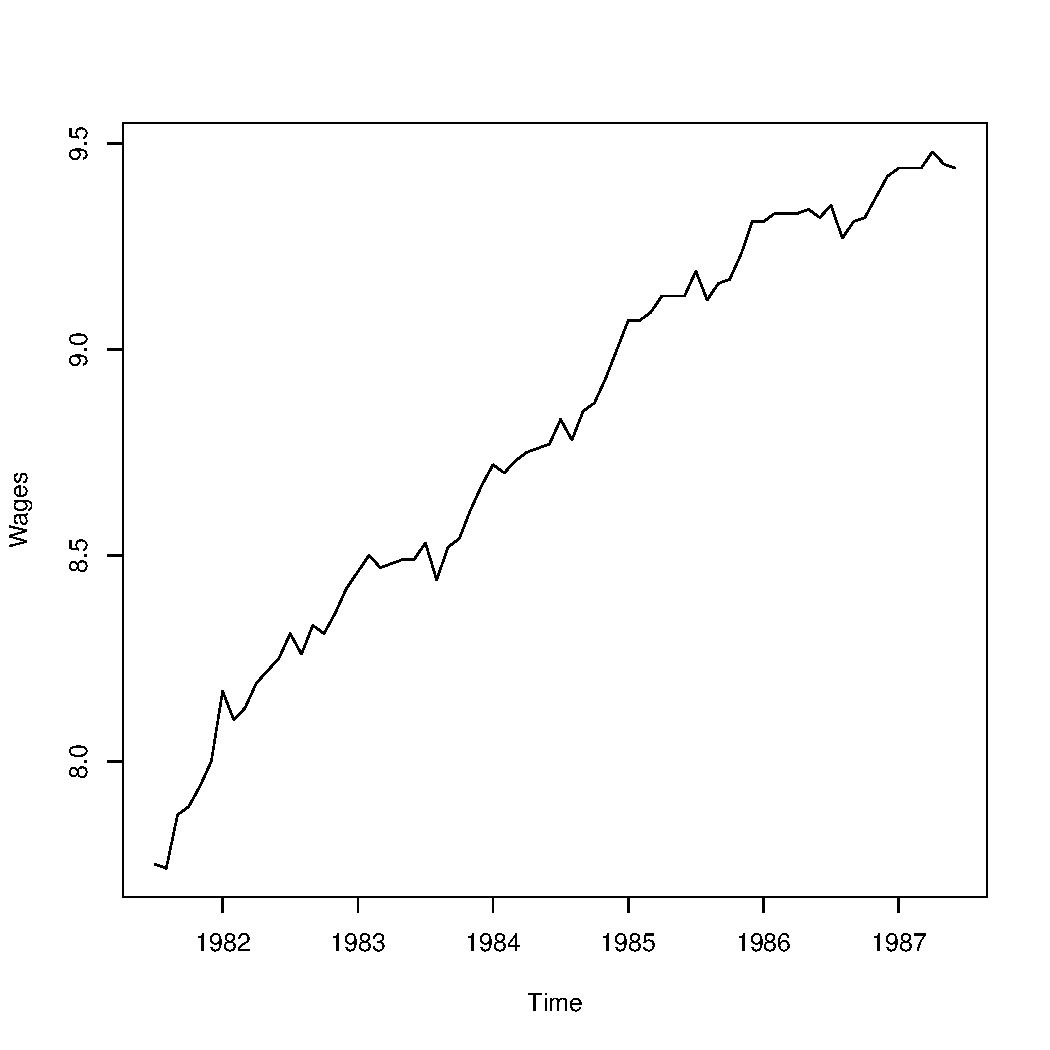
\includegraphics[width=.85\linewidth]{plot3_a_raw}
    \caption{Time series plot of wages.}
    \label{fig:plot3a}
    \end{subfigure}
    \begin{subfigure}{.5\textwidth}
        \centering
        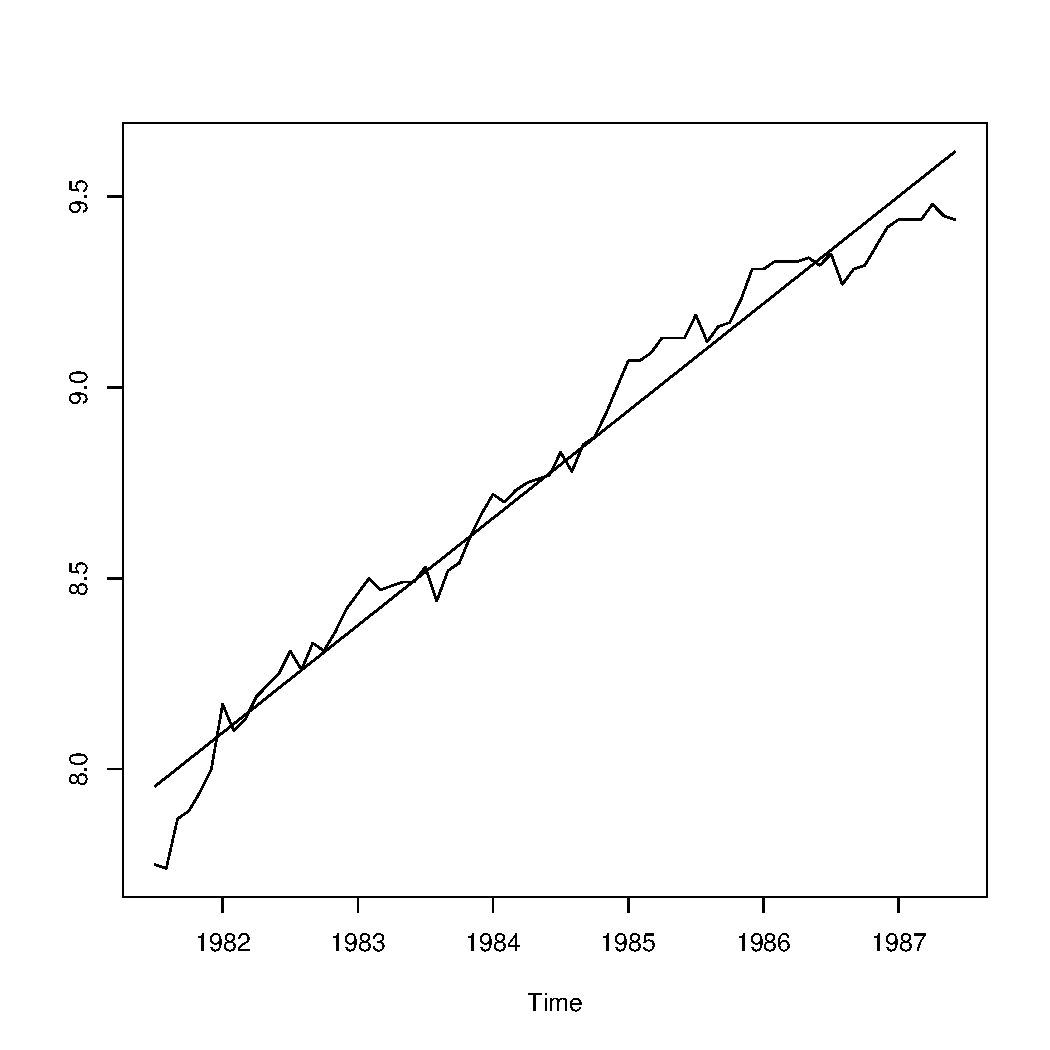
\includegraphics[width=.85\linewidth]{plot3_b_lin_fit}
        \caption{Linear regression, $\hat{\expect}(X_t)=7.93144 + 0.02342 t$.}
        \label{fig:plot3b}
    \end{subfigure}

    \begin{subfigure}{.5\textwidth}
    \centering
    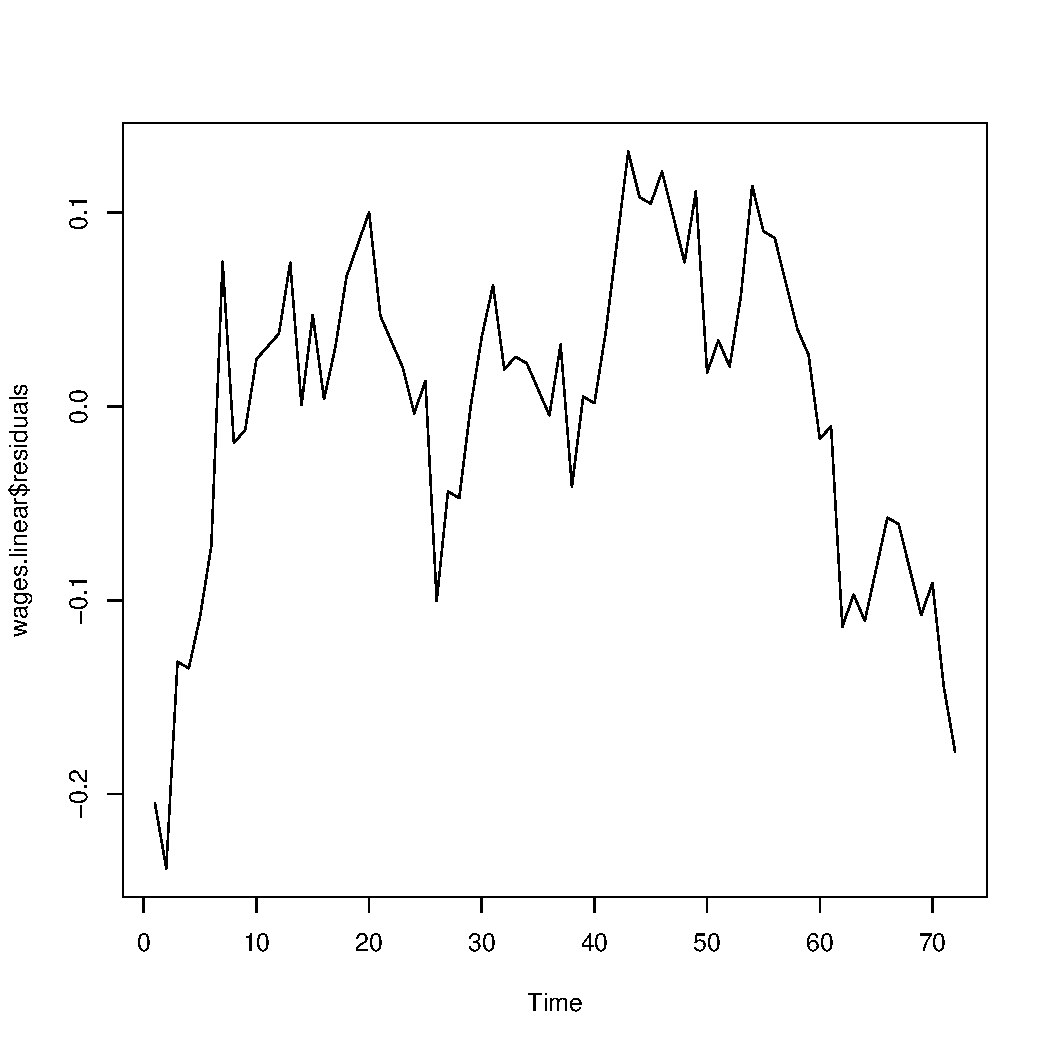
\includegraphics[width=.85\textwidth]{plot3_c_lin_resid}
    \caption{Linear regression residuals of the wages times series.}
    \label{fig:plot3c}
    \end{subfigure}
    \begin{subfigure}{.5\textwidth}
    \centering
    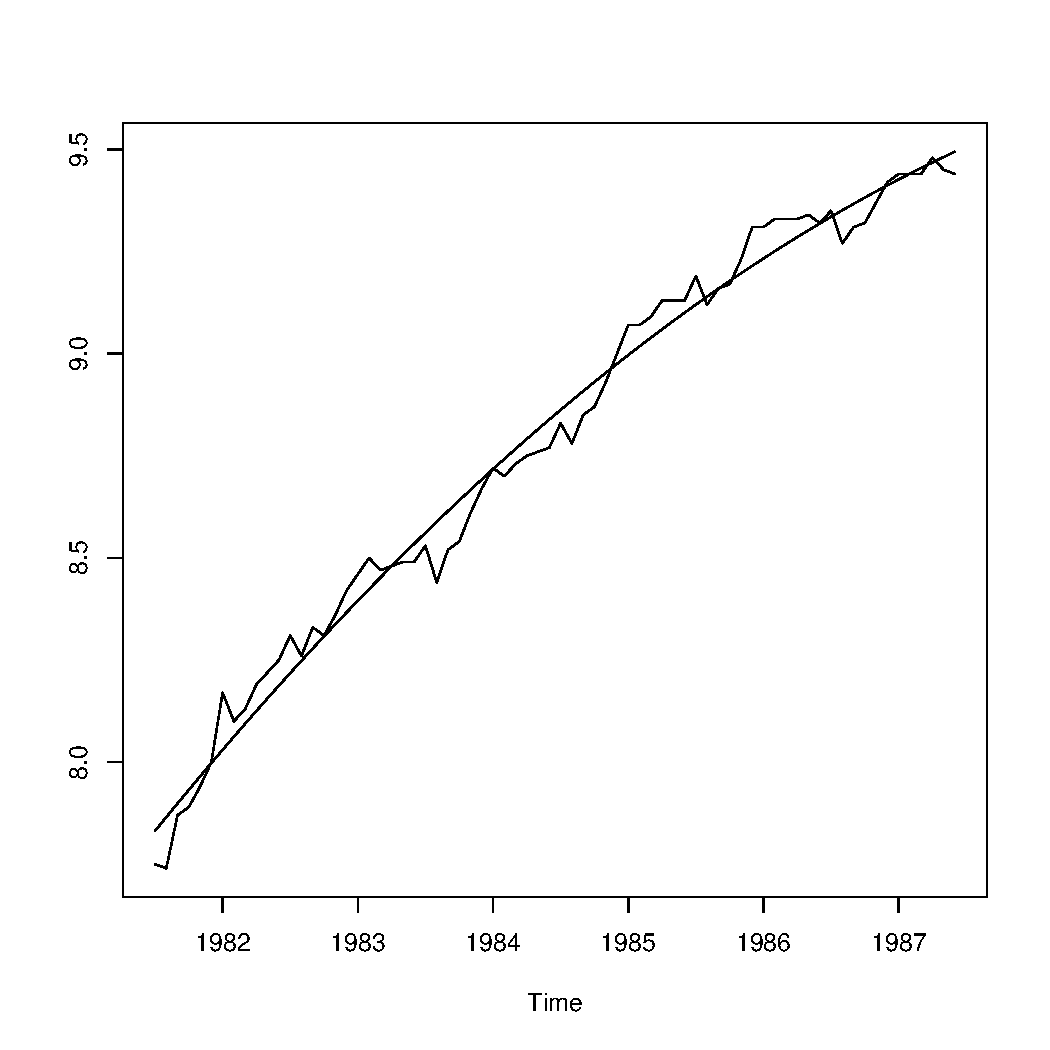
\includegraphics[width=.85\linewidth]{plot3_d_qd_fit}
    \caption{Quadratic regression, $\hat{\expect}(X_t) \coloneqq 7.7974363 + 0.0342882 t - 0.0001488 t^2$}
    \label{fig:plot3d}
    \end{subfigure}

    \begin{subfigure}{.5\textwidth}
    \centering
    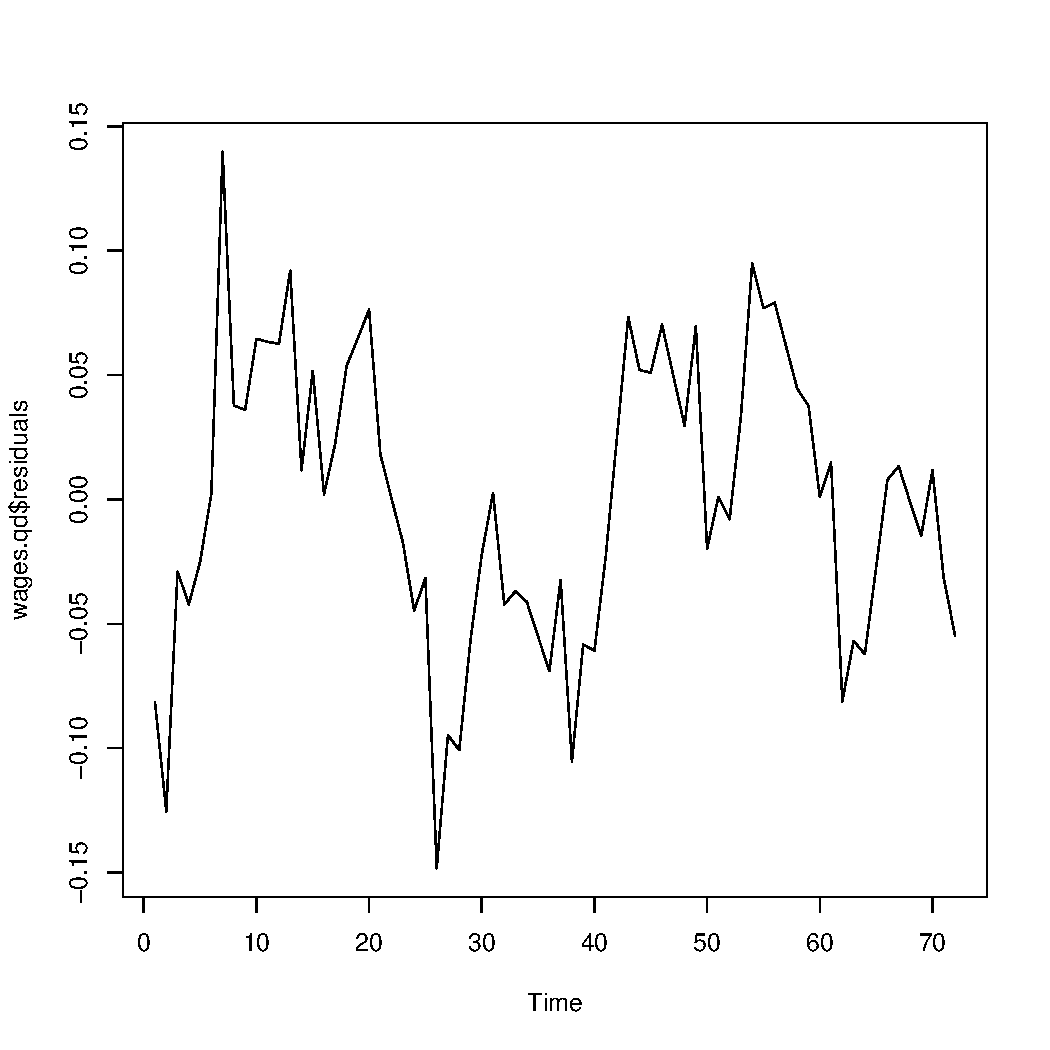
\includegraphics[width=.85\linewidth]{plot3_e_qd_resid}
    \caption{Quadratic regression residuals of the wages times series.}
    \label{fig:plot3e}
    \end{subfigure}
    \caption{Plots for problem $3$}
    \end{figure}

    \item[(c)] The linear residuals are plotted in fig~\ref{fig:plot3c}.
    What stands out about this plot is the middle region has mostly positive residuals, meaning that
    most of these data points are below the line of best fit, and the end points have negative residuals,
    suggesting that most of these points are below the line of best fit.
    In other words, the residuals are correlated.
    Also, near the far left and far right of the plot, we see some outliers which take on
    relatively large negative values compared to the rest.
    
        
    \item[(d)] The quadratic regression of best fit to the \emph{wages} time series dataset is given by
    \begin{equation}
        \hat{\expect}(X_t)=7.7974363 + 0.0342882 t - 0.0001488 t^2\,.
    \end{equation}
    We plot the wages time seres with this line of best fit in fig~\ref{fig:plot3d}.
    
    \item[(e)] The quadratic residuals are plotted in fig~\ref{fig:plot3e}.
    Unlike the linear regression line of best fit, the residuals are more uniformly centered
    around the mean and exhibit less correlation.
    These resdiuals seem to better model the concept of white noise.
    
\end{enumerate}

\end{document}
